\chapter{Performance}


\section{zero-cost in Rust}

Das Typsystem in Rust ermöglicht viele sogenannte zero-cost-Abstraktionen. Da\-durch kann der Code in Rust leserlich und überschaubar gestaltet werden, ohne dabei auf bestimmte Aspekte zu achten, die in anderen Programmiersprachen für einen Performanceverlust sorgen würden.

Folgender Code zeigt eine zero-cost-Abstraktion in Rust\cite{ZeroCost}:

\begin{lstlisting}
    struct Point2D {
        x: f64,
        y: f64,
    }
    
    impl Point2D {
        fn move_right(self, distance: f64) -> Point2D {
            Point2D {
                x: self.x + distance,
                y: self.y,
            }
        }
    }
    
    fn do_stuff(input: f64) -> f64 {
        let p1 = Point2D{ x: 3.0, y: 7.0 };
        let p2 = p1.move_right(input);
        p2.x
    }
\end{lstlisting}

Die Funktion \verb"do_stuff" bekommt eine Zahl, addiert sie mit \verb"3" und gibt diese wieder zurück. Im Code wurde dazu eine Struktur \verb"Point2D" mit der Funktion \verb"move_right" verwendet. Der Compiler erkennt, dass der Code der Funktion auf eine einfache Addition ver\-kürzt werden kann:

\begin{lstlisting}
    fn do_stuff(input: f64) -> f64 {
        3.0 + input
    }
\end{lstlisting}

Ein anderes Beispiel ist die Verwendung von Traits als Input für Funktionen:

\begin{lstlisting}
    trait Logger {
        fn error(&self, message: &str);
        fn info(&self, message: &str);
    }
    
    struct NullLogger {}
    
    impl Logger for NullLogger {
        fn error(&self, message: &str) {}
        fn info(&self, message: &str) {}
    }
    
    struct PrintLogger {}
    
    impl Logger for PrintLogger {
        fn error(&self, message: &str) {
            println!("ERROR: {}", message);
        }
        fn info(&self, message: &str) {
            println!("INFO: {}", message);
        }
    }
    
    fn log_example(logger: &dyn Logger) {
        logger.info("example info");
        logger.error("example error");
    }
\end{lstlisting}

Hier weiß Rust nicht, welche Art von Logger die Funktion \verb"log_example" benutzt. Die Optimierung der Funktion wird verhindert, da der Compiler erst zur Laufzeit wissen kann, wie die Funktionen \verb"logger.info" und \verb"logger.error" implementiert sind. Siehe \glqq dynamic dispatch\grqq{} in \autoref{dynamicdispatch}.

Mithilfe von generischen Funktionen können solche Optimierungen dennoch vorgenommen werden, da der Compiler für jede Art von Logger eine eigene Funktion erstellt, also \glqq static dispatch\grqq{} verwendet. Die generische Funktion könnte so aussehen:

\begin{lstlisting}
    fn log_example<L: Logger>(logger: &L) {
        logger.info("example info");
        logger.error("example error");
    }
\end{lstlisting}

Der Vorteil der Benutzung von generischen Funktionen besteht darin, dass Rust mehr Optimierungen vornehmen kann. Der Nachteil ist jedoch, dass die ausführbaren Binärdateien mehr Speicherplatz benötigen und das Kompilieren länger dauert.


\section{Benchmark-Tests}

Um festzustellen, wie performant Rust-Programme im Verhältnis zu anderen Spra\-chen laufen, können verschiedene Arten von Programmen ausgeführt und ge\-mes\-sen werden. In diesem Kapitel werden Daten aus dem Computer Language Benchmarks Game\footnote{https://benchmarksgame-team.pages.debian.net/benchmarksgame/} zitiert. Die Programme können von Usern hochgeladen werden und sind im Internet frei einsehbar. Sie wurden so programmiert, dass sie übliche Mittel der jeweiligen Sprache verwenden. Beispielsweise wird in C++ der \verb"new" Operator verwendet.

In den Balkendiagrammen ist Rust 100\% und die Prozentzahlen für C und C++ werden von den Ergebnissen aus Rust berechnet.

\hspace{1cm}

\begin{table}[htbp]
\centering
\begin{tabular}{|l|l|}
\hline
\rule[-1ex]{0pt}{2.5ex} \multirow{2}{*}{Rust} & rustc 1.35.0 (3c235d560 2019-05-20) \\ & LLVM version 8.0 \\
\hline
\rule[-1ex]{0pt}{2.5ex} C gcc & gcc (Ubuntu 8.3.0-6ubuntu1) 8.3.0 \\
\hline
\rule[-1ex]{0pt}{2.5ex} C++ g++ & g++ (Ubuntu 8.3.0-6ubuntu1) 8.3.0 \\
\hline
\end{tabular}
\caption{Compiler der Benchmark-Tests}
\end{table}

\subsection{Die Benchmarkprogramme}

\paragraph{binary trees}

In diesem Test geht es darum, einen vollständigen Binärbaum zu erstellen, den Baum \glqq herunterzuklettern\grqq{} und dabei die Knotenpunkte zu zählen und den Baum anschließend vom Speicher zu löschen.

\paragraph{fannkuch-redux} Eine Permutation von \{1,...,n\}, z. B. \{4,2,1,5,3\}. Die erste Zahl ist 4, es sollen also die ersten 4 Elemente getauscht werden. Das wird so oft wiederholt bis die 1 an der ersten Stelle ist: \{5,1,2,4,3\} \{3,4,2,1,5\} \{2,4,3,1,5\} \{4,2,3,1,5\} \{1,3,2,4,5\}.

\paragraph{fasta} Generierung von DNA-Sequenzen durch Kopieren aus gegebenen Sequenzen und Zufallszahlen. Dabei werden lineare und binäre Suchfunktionen verwendet.

\paragraph{k-nucleotide} Eine Hash-Tabelle wird zum Zählen von Vorkommen bestimmter Zeichenketten aus einer DNA-Sequenz benutzt.

\paragraph{mandelbrot} Ein Mandelbrot wird auf eine $N*N$ Bitmap geplottet.

\paragraph{n-body} Die Modellierung von Umlaufbahnen von Gasriesen mit einem symplektischen Integrator, also die Bewegung von Partikeln in einem Raum, dessen Masse von einem einzelnen Objekt dominiert wird.

\paragraph{pidigits} Berechnung von Pi mithilfe von Langzahlarithmetik.

\paragraph{regex-redux} Reguläre Ausdrücke anwenden um Übereinstimmungen zu finden.

\paragraph{reverse-complement} Rückwärtskomplement einer DNA-Sequenz berechnen.

\paragraph{spectral-norm} Berechnung der Spektralnorm einer Matrix.

\newpage

\subsection{Ausführungszeit}

\vspace{-0.9cm}

\begin{figure}[htbp]
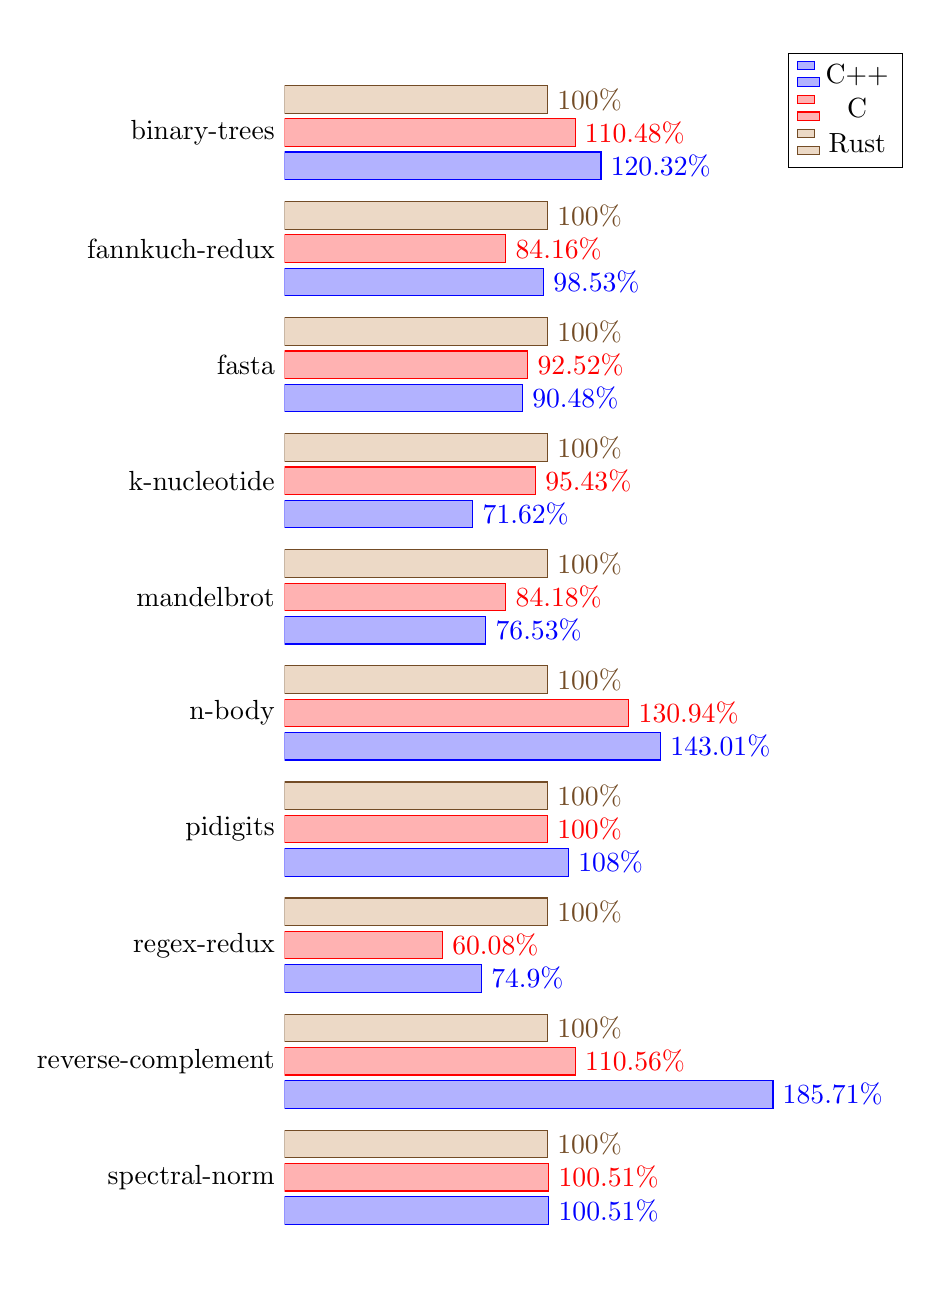
\begin{tikzpicture}
\begin{axis}[
    xbar,
    width = \textwidth-71.9pt,
    height = 17.5cm,
    y axis line style = { opacity = 0 },
    axis x line = none,
    xmin = 0,
    xmax = 240,
    tickwidth = 0pt,
    symbolic y coords = {spectral-norm,reverse-complement,regex-redux,pidigits,n-body,mandelbrot,k-nucleotide,fasta,fannkuch-redux,binary-trees},
    nodes near coords={\pgfmathprintnumber\pgfplotspointmeta\%},
]
\addplot coordinates {
    (120.32,binary-trees) (98.53,fannkuch-redux) (90.48,fasta) (71.62,k-nucleotide) (76.53,mandelbrot) (143.01,n-body) (108,pidigits) (74.9,regex-redux) (185.71,reverse-complement) (100.51,spectral-norm)
};
\addplot coordinates {
    (110.48,binary-trees) (84.16,fannkuch-redux) (92.52,fasta) (95.43,k-nucleotide) (84.18,mandelbrot) (130.94,n-body) (100,pidigits) (60.08,regex-redux) (110.56,reverse-complement) (100.51,spectral-norm)
};
\addplot coordinates {
    (100,binary-trees) (100,fannkuch-redux) (100,fasta) (100,k-nucleotide) (100,mandelbrot) (100,n-body) (100,pidigits) (100,regex-redux) (100,reverse-complement) (100,spectral-norm)
};
\legend{C++,C,Rust}
\end{axis}
\end{tikzpicture}
\caption{Ausführungszeit: Rust im Verhältnis zu C und C++}
\end{figure}

In diesen Tests läuft C schneller als C++, jedoch verfügt C++ über viele zu\-sätz\-liche Funktionen, die die Programmierung erleichtern können. Zusätzliche Funktionen besitzt auch die Sprache Rust, die durchschnittlich ähnlich wie C performt.

Besonders bei Berechnungen mit Fließkommazahlen im Test \glqq n-body\grqq{} ist Rust sehr performant, verliert aber bei anderen Aufgaben gegenüber C/C++. Dank der schnellen Ausführungszeit, eignet sich Rust für eingebettete Systeme.

Bei eingebetteten Systemen ist das Verhalten bei einer Panik nicht definiert. Das Verhalten bei einer Panik kann in Rust jedoch neu definiert werden. \cite{EmbeddedBook}

\newpage

\subsection{Speicherverbrauch}

\vspace{-0.9cm}

\begin{figure}[htbp]
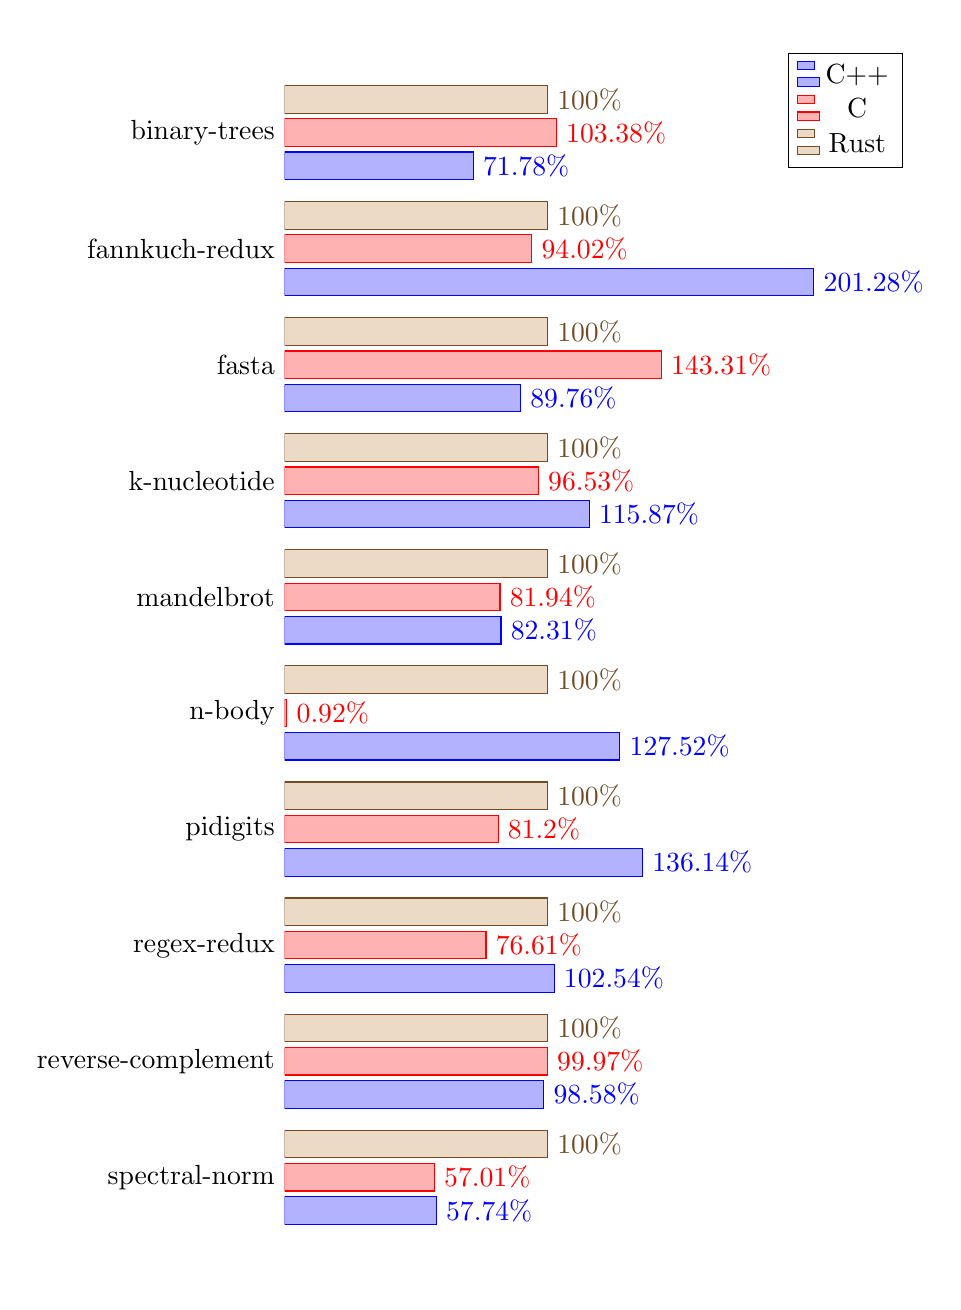
\begin{tikzpicture}
\begin{axis}[
    xbar,
    width = \textwidth-71.9pt,
    height = 17.5cm,
    y axis line style = { opacity = 0 },
    axis x line = none,
    xmin = 0,
    xmax = 240,
    tickwidth = 0pt,
    symbolic y coords = {spectral-norm,reverse-complement,regex-redux,pidigits,n-body,mandelbrot,k-nucleotide,fasta,fannkuch-redux,binary-trees},
    nodes near coords={\pgfmathprintnumber\pgfplotspointmeta\%},
]
\addplot coordinates {
    (71.78,binary-trees) (201.28,fannkuch-redux) (89.76,fasta) (115.87,k-nucleotide) (82.31,mandelbrot) (127.52,n-body) (136.14,pidigits) (102.54,regex-redux) (98.58,reverse-complement) (57.74,spectral-norm)
};
\addplot coordinates {
    (103.38,binary-trees) (94.02,fannkuch-redux) (143.31,fasta) (96.53,k-nucleotide) (81.94,mandelbrot) (0.92,n-body) (81.2,pidigits) (76.61,regex-redux) (99.97,reverse-complement) (57.01,spectral-norm)
};
\addplot coordinates {
    (100,binary-trees) (100,fannkuch-redux) (100,fasta) (100,k-nucleotide) (100,mandelbrot) (100,n-body) (100,pidigits) (100,regex-redux) (100,reverse-complement) (100,spectral-norm)
};
\legend{C++,C,Rust}
\end{axis}
\end{tikzpicture}
\caption{Speicherverbrauch: Rust im Verhältnis zu C und C++}
\end{figure}

In C kann dank der Low-Level-Orientierung viel Speicher eingespart werden. Jedoch gehen hier die Ergebnisse weit auseinander, wie z. B. bei den Tests \glqq fannkuch-redux\grqq{} und \glqq n-body\grqq{}.

Rust benötigt in den meisten Fällen nicht auffallend viel Speicher und ist dadurch als Systemprogrammiersprache geeignet.

% \newpage

% \subsection{CPU-Auslastung}

% \begin{figure}[htbp]
% \begin{tikzpicture}
% \begin{axis}[
%     xbar,
%     width = \textwidth-71.9pt,
%     height = 18cm,
%     y axis line style = { opacity = 0 },
%     axis x line = none,
%     xmin = 0,
%     xmax = 240,
%     tickwidth = 0pt,
%     symbolic y coords = {spectral-norm,reverse-complement,regex-redux,pidigits,n-body,mandelbrot,k-nucleotide,fasta,fannkuch-redux,binary-trees},
%     nodes near coords={\pgfmathprintnumber\pgfplotspointmeta\%},
% ]
% \addplot coordinates {
%     (89.01,binary-trees) (101.03,fannkuch-redux) (102.85,fasta) (99.35,k-nucleotide) (100.76,mandelbrot) (96.19,n-body) (103.96,pidigits) (150,regex-redux) (91.18,reverse-complement) (99.75,spectral-norm)
% };
% \addplot coordinates {
%     (90.93,binary-trees) (101.03,fannkuch-redux) (125.63,fasta) (105.48,k-nucleotide) (100.76,mandelbrot) (96.19,n-body) (114.85,pidigits) (145.68,regex-redux) (133.53,reverse-complement) (99.75,spectral-norm)
% };
% \addplot coordinates {
%     (100,binary-trees) (100,fannkuch-redux) (100,fasta) (100,k-nucleotide) (100,mandelbrot) (100,n-body) (100,pidigits) (100,regex-redux) (100,reverse-complement) (100,spectral-norm)
% };
% \legend{C++,C,Rust}
% \end{axis}
% \end{tikzpicture}
% \caption{CPU-Auslastung: Rust im Verhältnis zu C und C++}
% \end{figure}
